\chapter{Antenna calculation and simulations}
\section{4NEC2}
As explained in the introduction, the 4NEC2 program is made by a radio amateur named Arie Voors\cite{4nec2}, with the goal of being a open source program to help other radio amateurs simulate antennas. This program is not the best of all programs, but as a open source tool and for what is needed in this thesis it will do the job. Some of the things that the program can do is: near and far field analysis, showing VSWR, gain, impedance, half-power beam width and antenna efficiency. The program can also analyze an antenna in different situation, such as: free-space, perfect ground and real ground. It can show a 3-dimensional picture of the radiation pattern for the antenna, but it can also plot the radiation pattern in 2-dimension, for the vertical an horizontal plane, as seen in figure 2.19 and 2.20. furthermore, it is capable of showing a smith chart and impedance matching an antenna to any given impedance, using either an L-filter, Pi-network or T-network. The downside of this program, is that it is hard to draw complex structures, such as a folded dipole or anything that is circular. Furthermore this the program can not simulate patch antennas, see section 2.6.6 \textit{Microstrip patch antenna}. It is not within the scope of this thesis to explain how to use the program, there are tutorials on the internet that explains how to use the program, moreover, there is a guide on the original website on how to use the program, see reference\cite{4NEC2Guide}. 

\begin{figure}[h!]
\centering
%\hspace*{-2.3cm}
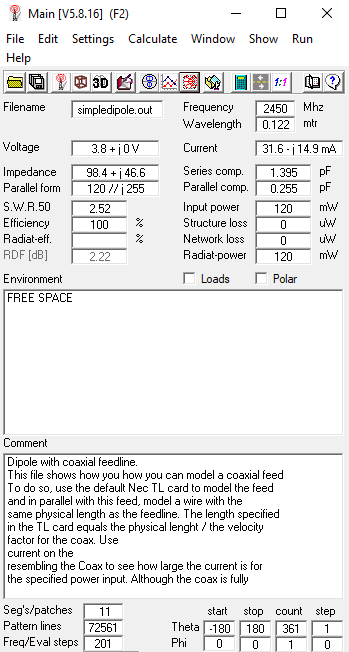
\includegraphics[scale=0.60]{figures/4nec2.PNG}
\caption{Showing the front page of the 4NEC2 program}
\end{figure}

\section{Yagi calculator}
The Yagi calculator is also an open source program made by a radio amateur, John Drew\cite{yagical}, with the goal of making it easier to quickly design and build a yagi antenna. This program does not simulate the antenna, but rather uses a template made by years of experimentation in the radio amateur world, even the front page of the program states that, see figure 3.2. The program is capable of calculating the size of the yagi-uda elements, the dimension of the driven element (folded dipole) and the distance between each elements, see section 2.6.7 \textit{Yagi-uda and cross-yagi-uda antennas}. It can calculate the half-power beam width, the gain for each director added. If a coaxial cable is specified the program can calculate the length of the matching stub, to match the yagi antenna to an impedance of $50\Omega$.

\begin{figure}[h!]
\centering
%\hspace*{-2.3cm}
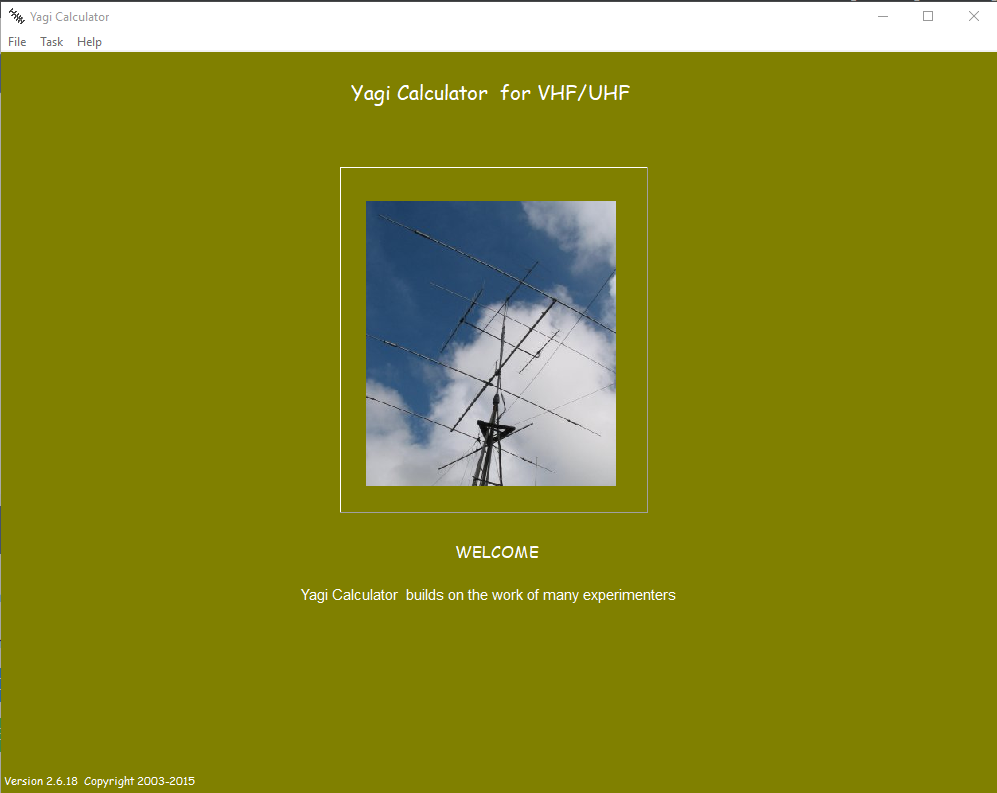
\includegraphics[scale=0.5]{figures/YagiCalculator.PNG}
\caption{Showing the front page of the Yagi calculator program}
\end{figure}

\section{Dipole}
%length of dipole each arm
% show the simulations

\section{Quaterwave monopol}
%length of Quaterwave monopol each arm
% show the simulations and results
\section{Helical}
%use the matlab code in conjunction with the theory part

\section{Yagi-uda and cross yagi-uda}
%% use yagi antena software and merge it with repport about cross-yagi antenna, DONT SIMULATE IT, since you are not using this type of antenna. 

\section{Partial conclusion}